\section{Diodes}\label{sec:Diodes}
A \nameref{def:Diode} is one of the basic building blocks for almost all analog circuit systems.

\begin{definition}[Diode]\label{def:Diode}
  A \emph{diode} is a 2-port non-linear circuit element.
  Its circuit symbol is shown in \Cref{fig:Diode_Circuit_Symbol}.
\end{definition}

\begin{figure}[h!tbp]
  \centering
  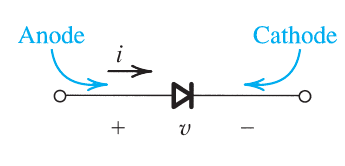
\includegraphics[scale=0.75]{./Diode_Circuit_Symbol.png}
  \caption{Diode Circuit Symbol \parencite[p.~177]{sedraTextbook7}}
  \label{fig:Diode_Circuit_Symbol}
\end{figure}

An \textbf{ideal diode} is one that behaves as a short-circuit when a voltage applied is forward-biased, and acts as an open-circuit with the voltage is reverse-biased.
The current-voltage characteristic is shown in \Cref{fig:Ideal_Diode_IV_Characteristic}.

\begin{figure}[h!tbp]
  \centering
  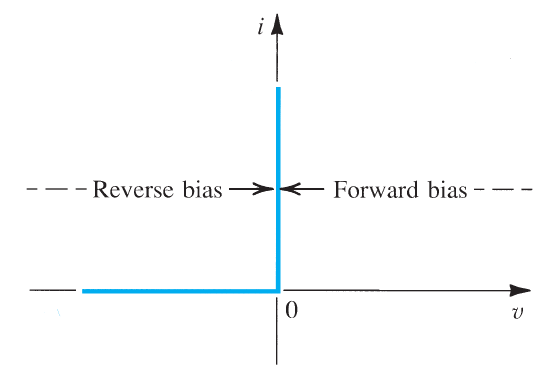
\includegraphics[scale=0.75]{./Ideal_Diode_IV_Characteristic.png}
  \caption{Ideal Diode \DCCurrent{}-\DCVoltage{} Characteristic \parencite[p.~177]{sedraTextbook7}}
  \label{fig:Ideal_Diode_IV_Characteristic}
\end{figure}

\subsection{Terminal Characteristics of Junction Diodes}\label{subsec:Terminal_Characteristics_Junction_Diodes}
A \textbf{junction diode} is a \nameref{def:Diode} built using a \PNJunction{}.
In this case, there are three distinct regions in the characteristic curve:
\begin{enumerate}[noitemsep]
\item \nameref{subsubsec:Diode_Forward-Bias_Region}, where $\Voltage > 0$.
\item \nameref{subsubsec:Diode_Reverse-Bias_Region}, where $\Voltage < 0$.
\item \nameref{subsubsec:Diode_Breakdown_Region}, where $\Voltage < - \ReverseBreakdownVoltage$.
\end{enumerate}

\subsubsection{The Forward-Bias Region}\label{subsubsec:Diode_Forward-Bias_Region}
The forward-bias region is the one where the terminal voltage $\Voltage$ is positive.

In the forward region, we can approximate the current-voltage relationship by using \Cref{eq:pn-Junction-Current-Voltage_Relation-Simple}, with minor modifications, as seen in \Cref{eq:Diode_Forward-Bias-IV_Relationship}.

\begin{equation}\label{eq:Diode_Forward-Bias-IV_Relationship}
  \Current = \SaturationCurrent \left( e^{\frac{\Voltage}{\ThermalVoltage}} - 1 \right)
\end{equation}

There is a slightly \textbf{more} modified version, in \Cref{eq:Diode_Forward-Bias-IV_Relationship-n}

\begin{equation}\label{eq:Diode_Forward-Bias-IV_Relationship-n}
  \Current = \SaturationCurrent \left( e^{\frac{\Voltage}{n \ThermalVoltage}} - 1 \right)
\end{equation}

$n$ has a value between 1 and 2.
$n$ is a number that depends on the material and physical structure of the diode.
From here-on-out, we assume that $n = 1$.
However, there may be cases when you should use a different $v$ value instead.


%%% Local Variables:
%%% mode: latex
%%% TeX-master: "../ECE_311-Engineering_Electronics-Reference_Sheet"
%%% End:
